\documentclass{article}

\usepackage{amsmath, amssymb, amsfonts}
\usepackage{graphicx}
\usepackage{fancyvrb}

\newcommand{\R}{\mathbb{R}}
\newcommand{\ol}{\overline}

\author{Matthew Dupraz}
\title{Homework 11}

\begin{document}

\maketitle

\subsection*{(a)}

We want to find $x_1, x_2 \in \R$ such that
$\sum_{i = 1}^m(x_1 + x_2 t_i - y_i)^2$ is minimized.

We have that $\sum_{i=1}^m(x_1 + x_2t_i - y_i)^2 = 
\|Ax - y\|_2^2$, where
\begin{equation*}
	A = 
	\begin{bmatrix}
		1 & t_1 \\
		1 & t_2 \\
		\vdots & \vdots \\
		1 & t_m
	\end{bmatrix},
	x =
	\begin{bmatrix}
		x_1 \\
		x_2
	\end{bmatrix},
	y =
	\begin{bmatrix}
		y_1 \\
		\vdots \\
		y_m
	\end{bmatrix}
\end{equation*}
It follows that this problem is equivalent to
finding $x$, which minimizes $\|Ax - y\|_2^2$, which is
in turn equivalent to finding the solutions of
\begin{equation*}
	A^TAx = A^Ty
\end{equation*}

Define $\ol{t} = \frac{1}{m}\sum_{i = 1}^m t_i$,
$\ol{t^2} = \frac{1}{m}\sum_{i = 1}^m t_i^2$,
$\ol{y} = \frac{1}{m}\sum_{i = 1}^m y_i$,
$\ol{ty} = \frac{1}{m}\sum_{i = 1}^m t_iy_i$,
then we have that
\begin{equation*}
	A^TA =
	\begin{bmatrix}
		m & m \cdot \ol{t} \\
		m \cdot \ol{t} & m \cdot \ol{t^2}
	\end{bmatrix}
	= m
	\begin{bmatrix}
		1 & \ol{t} \\
		\ol{t} & \ol{t^2}
	\end{bmatrix}
\end{equation*}
and
\begin{equation*}
	A^Ty =
	\begin{bmatrix}
		m \cdot \ol{y} \\
		m\cdot \ol{ty}
	\end{bmatrix}
	= m
	\begin{bmatrix}
		\ol{y} \\
		\ol{ty}
	\end{bmatrix}
\end{equation*}

\subsection*{(b)}

And so the equation $A^TAx = Ay$ is equivalent to
\begin{equation*}
	\begin{bmatrix}
		1 & \ol{t} \\
		\ol{t} & \ol{t^2}
	\end{bmatrix}
	\begin{bmatrix}
		x_1 \\
		x_2
	\end{bmatrix}
	=
	\begin{bmatrix}
		\ol{y}\\
		\ol{ty}
	\end{bmatrix}
\end{equation*}
We isolate $x_1$ and $x_2$:
\begin{align*}
	&	
		\begin{cases}
			x_1 = \ol{y} - x_2\ol{t} \\
			x_2\ol{t^2} = \ol{ty} - x_1\ol{t}
		\end{cases}\\
	\iff &
		\begin{cases}
			x_1 = \ol{y} - x_2\ol{t} \\
			x_2\ol{t^2} = \ol{ty} - (\ol{y} - x_2\ol{t})\ol{t}
		\end{cases}\\
	\iff & 
		\begin{cases}	
			x_1 = \ol{y} - x_2\ol{t} \\
			x_2 = \frac{\ol{ty} - \ol{t}\cdot\ol{y}}{\ol{t^2} 
			- \ol{t}^2}
		\end{cases}\\
	\iff &
		\begin{cases}
			x_1 = \frac{\ol{t^2}\cdot\ol{y} - \ol{t}\cdot\ol{ty}}
			{\ol{t^2} - \ol{t}^2} \\
			x_2 = \frac{\ol{ty} - \ol{t}\cdot\ol{y}}{\ol{t^2}
			- \ol{t}^2}
		\end{cases}
\end{align*}

\subsection*{(c)}

Below follows the code I used for part (c):
\begin{Verbatim}[frame = single,
	label = \textsc{Matlab} code for part (c)]
% We define the functions that yield x_1 and x_2 from y and t
x_1 = @(t, y) (mean(t.^2)*mean(y) - mean(t)*mean(t.*y)) ...
				/ (mean(t.^2) - mean(t)^2);
x_2 = @(t, y) (mean(t.*y) - mean(t)*mean(y)) ...
				/(mean(t.^2) - mean(t)^2);

% Part (c)
load data.mat;

t = data(:, 1);
y = data(:, 2);

a = x_1(t, y);
b = x_2(t, y);

disp('Part (c)')
fprintf('x_1 = %g\n', a);
fprintf('x_2 = %g\n', b);

subplot(1, 3, 1);

scatter(t, y, 'filled');
hold on;

ts = [min(t), max(t)];
plot(ts, a + b*ts, 'LineWidth', 2);

set(gca, 'FontSize', 14);
grid on;
\end{Verbatim}

We obtained the following values for $x_1$ and $x_2$:
\begin{align*}
	x_1 &= 10.6692\\
	x_2 &= 1.00435
\end{align*}

Below follows the scatter plot with the data points, along
with the calculated best fit line

\begin{center}
	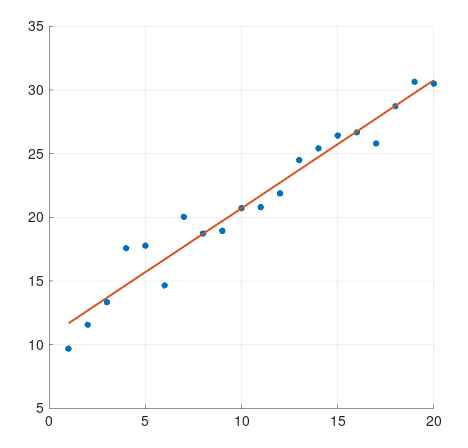
\includegraphics[width=0.5\textwidth]{figure1.png}
\end{center}

\subsection*{(d)}

Below follows the code I used for part (d):
\begin{Verbatim}[frame = single,
	label = \textsc{Matlab} code for part (d)]
% Part (d)
f = @(t) 1./(2 + t);
t = [-1; 0; 1];
y = f(t);

a = x_1(t, y);
b = x_2(t, y);

disp('Part (d)')
fprintf('x_1 = %g\n', a);
fprintf('x_2 = %g\n', b);

subplot(1, 3, 2);

scatter(t, y, 'filled');
hold on;

ts = linspace(-1, 1, 100);
plot(ts, f(ts), 'LineWidth', 2);

ts = [-1, 1];
plot(ts, a + b*ts, 'LineWidth', 2);

set(gca, 'FontSize', 14);
grid on;
\end{Verbatim}

We obtained the following values for $x_1$ and $x_2$:
\begin{align*}
	x_1 &= 0.611111\\
	x_2 &= -0.333333
\end{align*}

Below follows the plot obtained:
\begin{center}
	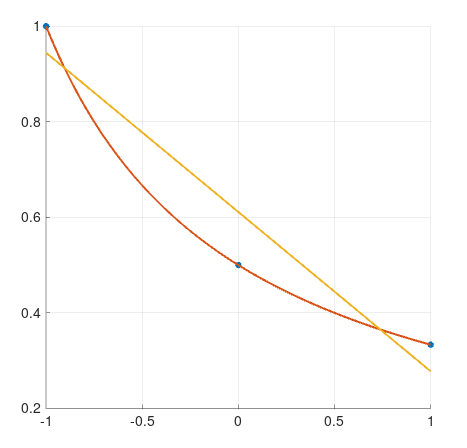
\includegraphics[width=0.5\textwidth]{figure2.png}
\end{center}

\subsection*{(e)}

Below follows the code I used for part (e):
\begin{Verbatim}[frame = single,
	label = \textsc{Matlab} code for part (e)]
% Part (e)

t = (1:10)';
y = (1:10)';

a = x_1(t, y);
b = x_2(t, y);

disp('Part (e)')
fprintf('x_1 = %g\n', a);
fprintf('x_2 = %g\n', b);

y(10) = 5;
a = x_1(t, y);
b = x_2(t, y);

subplot(1, 3, 3);

scatter(t, y, 'filled');
hold on;

ts = [1, 10];
plot(ts, a + b*ts, 'LineWidth', 2);

f = @(x) norm(x(1) + x(2)*t - y, 1);
x = fminsearch(f, [0, 0]);
plot(ts, x(1) + x(2)*ts, '--', 'LineWidth', 2);

set(gca, 'FontSize', 14);
grid on;
\end{Verbatim}

We got $x_1 = 0$ and $x_2 = 1$ for the unperturbed data, so in this
case the formula we found in $(b)$ indeed exactly recovers data.

Below follows the plot obtained:
\begin{center}
	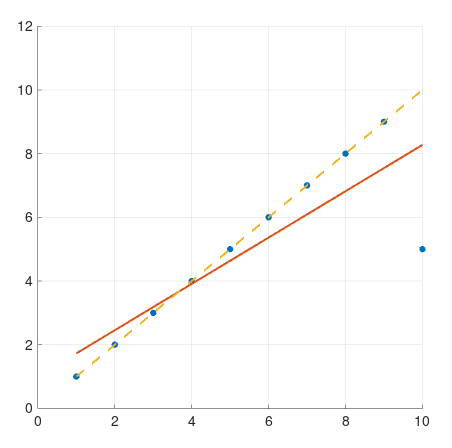
\includegraphics[width=0.5\textwidth]{figure3.png}
\end{center}
The full line corresponds to the parameters obtained with the
formula from part (b). The dashed line corresponds to the
parameters obtained using \texttt{fminsearch} to minimize the
absolute error function. We see that when we minimize the absolute
error, instead of quadratic, the result is much less affected
by outliers.

\end{document}
